% You can write any comments you want as long as there is a percentage sign at the beginning. This won't appear in your document.

\documentclass[12pt]{article}
%	options include 12pt or 11pt or 10pt
%	classes include article, report, book, letter, thesis, with 'article' being the default layout

\usepackage{amssymb,amsmath,textcomp} %These are optional packages you can install which gives you more mathematical symbols to play with

\usepackage{graphicx,subfig,enumerate,rotating,listings}
\graphicspath{{img/}}



\title{Introduction to Vision and Robotics\\Robotics Practical: Line Follower}
\author{Dylan Angus, Matthew Martin}
\date{\today}

%%%%%%%%%%%%%%%%%%%%%%%%%%%%%%%%%%%%

% OUTLINE

% Introduction
%	Descirption of the problem
% 	Overview of our approach
%		Used a PID controller to handle a lot of the movement
%		Did some odometry testing to assist with other movements

% Methods
%	Testing, getting to know the robot
%		clicks to cm conversion
%		etc
%	Setting up the odometry
%
%	Describe in detail how the important parts of each task were accomplished
%		general line following
%			tuning the PID
%		navigating from one line to the next in the broken line
%			using PID break case
%		navigating around the object
%			detection
%			turning
%			tuning PID with the goal distance
%				problems with the sonar pointing at the corner of the box - it wan't reading that as being close to the robot due to what we talked about in lecture about donar getting deflected not perpendicularly
%			finding the line again

% Results
%	Data from testing of robot
%		PID graphs for line following and obstacle avoiding
%	Data from reliability of odometry system

% Discussion
%	Successes
%	Limitations
%	Problems/Improvements


%%%%%%%%%%%%%%%%%%%%%%%%%%%%%%%%%%%%%

\begin{document}

%%%%%%%%%%%%%%%%%
% CUSTOM COMMANDS
\newcommand{\code}[1]{
	\lstinline[basicstyle=\ttfamily]|#1|
}

%%%%%%%%%%%%%%%%%

\maketitle

\section{Introduction}

The purpose of this practical is to learn about controlling a four-wheeled robot within a known environment. We used Lego's EV3 Python toolkit, assembling our own robot and developing all the robot code in Python. The robot is meant to accomplish three tasks:

\begin{itemize}
	\item Follow a curved line from beginning to end
	\item Follow a set of broken and staggered lines, going from one line to the next
	\item Complete a lap of a closed circuit while circumventing an object placed in the path of the robot
\end{itemize}

\section{Getting to know our robot}

We approached these tasks in a series of steps. First, we tried to gain familiarity with the operation of the robot by performing several tests on it to see its movement based on commands that were sent to it. Then, using this information, we tried developing a system of odometry and dead-reckoning. Finally, we solved the tasks sequentially, as each subsequent task built on some of the methods developed in the prior task.

\subsection{Initial Testing}

We conducted several tests in order to get consistency in how the commands that were sent to the robot translate to actual distance moved in the world.

First, we ran the motors for a series of durations using \code{run\_to\_rel\_pos()} keeping the \code{duty\_cycle\_sp} parameter constant at 25\%. These durations were in the unit of tacho counts, which is how the rotary encoder inside the motor measures turns. We performed tests at 25\% power for tacho counts of 100 to 700, incremented by 50. See Figure \ref{fig:motor_distance} for this data. From these tests and the slope of the trend line observed, we concluded that for forward commands we can convert from centimeters to tacho counts by performing the following calculation:

\[tachoCounts=\frac{centimeters}{4.807090465}\].

Then we performed similar testing on the angle that the robot turned based on a series of commands. We measured the angle by reading the gyro sensor before the command and after the command. The motors were kept at 25\% power, and we turned one wheel forward and the other reverse to do an in-place rotation. See Figure \ref{fig:rotation_distance} for a plot of this data. We observed the following conversion from tacho counts to degrees:

\[tachoCounts=\frac{degrees}{0.4695354523}\].

These conversions proved useful in commanding our robot to move set distances or rotate a specific number of degrees, as the robot's performance was quite consistent (as is observable from the very high $R^2$ values).

\begin{figure}
	\subfloat[distance travelled versus tacho counts (clicks) commanded] {
		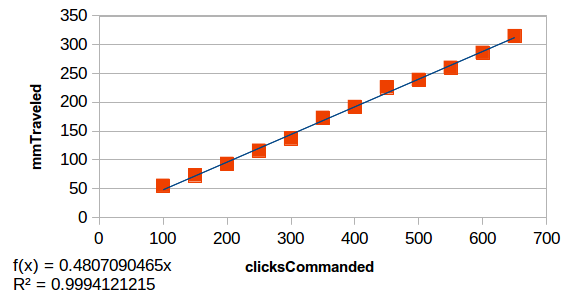
\includegraphics[width=\linewidth]{motor_distance}
		\label{fig:motor_distance}
	}
	\hfill
	\subfloat[angle turned versus tacho counts (clicks) commanded] {
		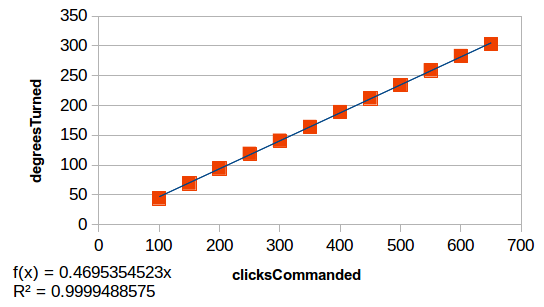
\includegraphics[width=\linewidth]{rotation_distance}
		\label{fig:rotation_distance}
	}

	\label{fig:distance_testing}
	\caption{These are two plots generated by a series of commands where a movement metric was recorded as the result of a number of tacho counts (clicks) commanded.}

\end{figure}

\subsection{Odometry and Dead Reckoning}

Initially, we attempted to make a full dead reckoning system. The resulting system basically worked but with too much error to be useful. Though we could have attempted to account for the error and make the system more accurate, the gain from having a working system did not outweigh the cost of testing and developing it as we were able to complete the tasks without it. Instead, it was settled on simply knowing the relation between wheel rotation and real-world distance and angular change. This was achieved through the testing described above. 

\section{Tasks}

\subsection{Methods}

Each of the three tasks built upon each other, beginning with simple line following.

\subsubsection{Line Following}

For line following, we used a PID controller. The overall idea was to set the goal of the PID controller to be the brightness value of the edge of the line. Therefore, the controller would constantly try to maintain that goal which would correspond to following the edge of the line. To normalize the readings fed to the PID controller, the raw readings from the color sensor had to undergo some calculations. Firstly, the raw output of the color sensor was capped so that it's values stayed in the range of 10 and 50 (we found the edge of the line to have a value of approximately 30). Those values were then shifted by thirty so that they were centered across 0. Finally, these values were fed to the mathematical function tanh so that the output was between -1 and 1. This information was sent as the current value to the PID each iteration. The goal of the PID was set to 0. Then, we did extensive tuning to achieve smooth results and steady-state accuracy.

Our tuning process consisted of roughly following the Ziegler-Nichols method, but mostly a lot of try-and-revise. The first set of relatively stable constants we settled on for line following were $K_p=4,K_i=2,K_d=8$. This resulted in our robot having consistent, but somewhat large oscillations, and good performance on turns. This corresponds to the blue line in Figure \ref{fig:pid_lines_a}. It can be seen that its oscillations around the goal (0) are fairly large and it never really settles to steady state. Next, we tried eliminating the integral term with the constants $K_p=6,K_i=0,K_d=2$. The performance of these constants were impressive on the straight part of the line, but disappointing on the curves. You can see the orange line in Figure \ref{fig:pid_lines_a} which plateaus at about 6 at the beginning and end of the plot. These are the periods when the robot was making a turn. However, during the straight section in between those turns we saw the robot achieve its steady state nicely.

With this knowledge, we thought that adding the $K_i$ and increasing the $K_p$ would correct for these errors and maintain some of that stability. We adjusted the constants to be $K_p=12,K_i=1,K_d=3$. Its performance on the straight line is not as good as the second set of constants we tried, but it had less overshoot than the first set as can be seen in the blue line in Figure \ref{fig:pid_lines_b}. We made some adjustments that we thought would account for this. The last iteration is the set of constants that we settled on, $K_p=6.5,K_i=0.825,K_d=3.0$. You can see in the red line in Figure \ref{fig:pid_lines_b} that it achieves steady state during the middle section (straight line), and has minimal oscillations on the curve. Its rise time in the curved sections of the line leave room for improvement, but we decided that these constants were the ones we would use for line following.

\begin{figure}
	\subfloat[the first two sets of constants for PID line following]{
		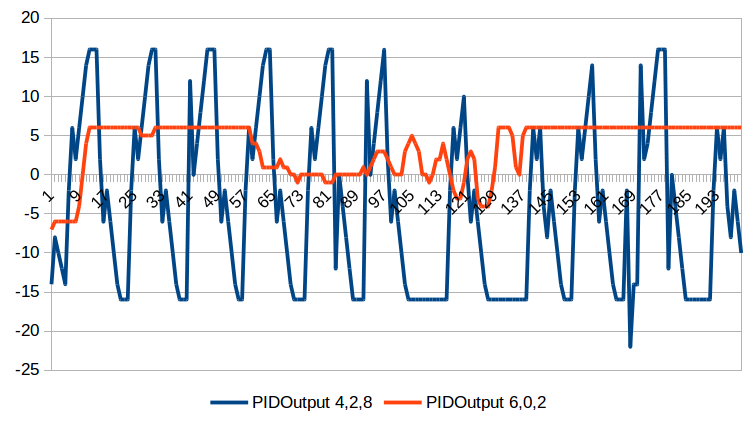
\includegraphics[width=\linewidth]{pid_line_a}
		\label{fig:pid_lines_a}
	}
	\hfill
	\subfloat[the second two sets of constants for PID line following]{
		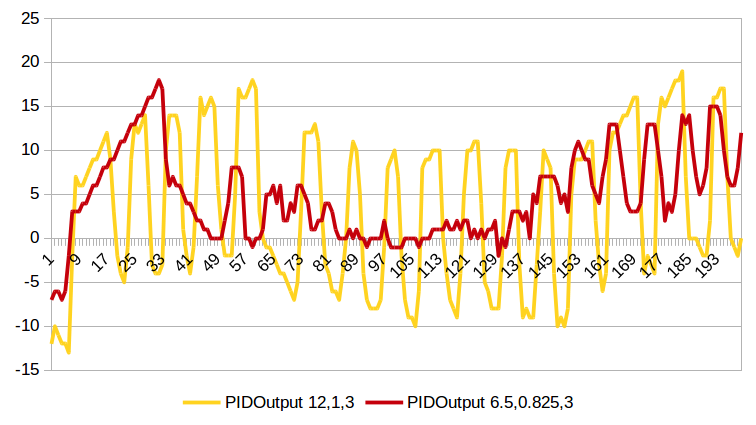
\includegraphics[width=\linewidth]{pid_line_b}
		\label{fig:pid_lines_b}
	}
	
	\caption{Overlaid plots of the four sets of constants for PID line following. The goal of the controller is 0.}
	\label{pid_lines}
\end{figure}

\subsubsection{Staggered line navigation}

Following the set of staggered lines proved not to be very difficult after developing a consistent PID controller for the line following. We had to make a few additions to the algorithm used for line following in order to traverse these lines. First, we made a strict breakout case for the line following by having a count increment whenever the robot was off the line, and reset when it was on the line. When the count got to some sufficiently large value we knew the robot had completed a line. Then depending on the number of lines it had completed, it turned right or left and drove forward until it found the next line. Then followed that one, and repeated the whole process until it completed all the lines.

\subsubsection{Obstacle avoidance}

This task required the robot to follow a line until it sees an obstacle, then go around said obstacle and find the line again. To do this the robot was programmed to use same the line following function that has been discussed until the sensor reading for the ultrasonic sensor fell below a threshold of 75 (7.5 cm). After falling below this threshold it turns ninety degrees on the spot then turns its servo ninety degrees the opposite direction towards the object. It then uses readings from the ultrasonic sensor to send to a PID controller which attempts to maintain a constant distance between the obstacle and the robot until it detects the line again. After seeing the line again the robot then returns to following the line.

The time-consuming aspect of this task was, again, tuning the PID controller for circumventing the object. We set the goal distance as 125 (12.5 cm), and set the robot to maintain that goal around the whole object. In order to remove noise from the sonar reading, which had a range of 2550, we capped those readings at 500. This helped because we wanted behavior to be consistent around the box regardless if the sonar was reading something irrelevant but that was closer than 2550 millimeters away. This improved the performance greatly, and we ended up using mostly the $K_p$ constant, with $K_i=0$ and $K_d$ equal to a small value. We found that with just $K_p$, the robot was turning too quickly and a small $K_d$ counteracted this nicely. See Figure \ref{fig:pid_object} for a plot of the error as it rounded the box.

\begin{figure}
	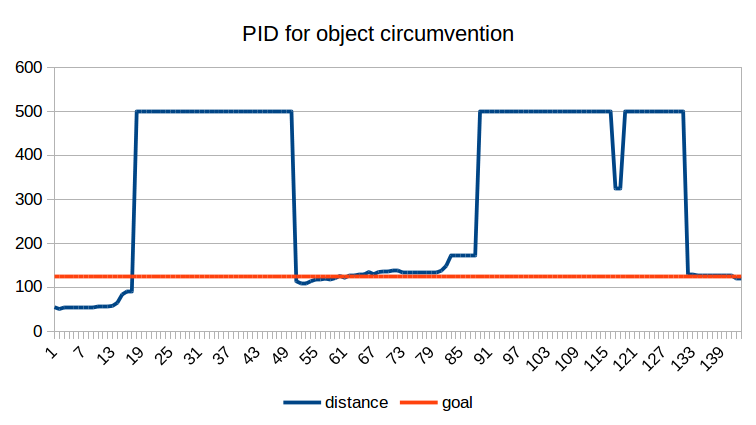
\includegraphics[width=\linewidth]{pid_object_outs}
	\caption{The results from tuning our PID controller for obstacle avoidance.}
	\label{fig:pid_object}
\end{figure}

\subsection{Results}

\subsubsection{Line Following}

The results of our line following PID controller on the actual path can be seen in Figure \ref{fig:taskA_plot}. This graph shows that our controller, although it experiences oscillations and never truly finds the steady state, is reliable and robust by not ever letting the error get too large.

\begin{figure}
	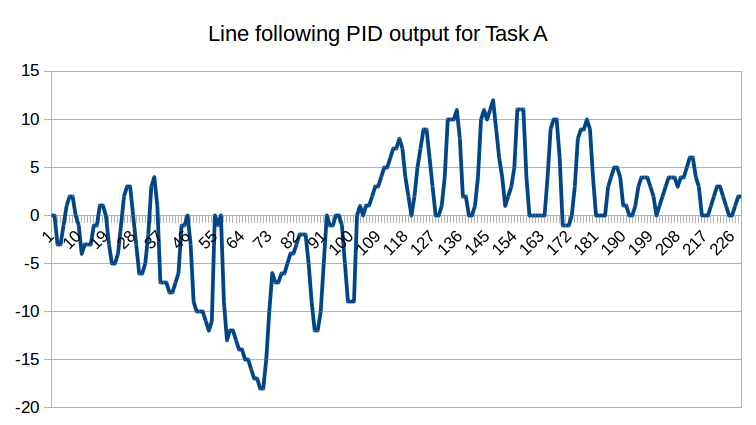
\includegraphics[width=\linewidth]{pid_taskA}
	\caption{The results from tuning our PID controller for Task A completion.}
	\label{fig:taskA_plot}
\end{figure}

\subsubsection{Staggered Line Navigation}

There are no unique results to discuss in the staggered line, since it uses the PID controller from Task A. We were happy with the consistency of the breakout case, as its accuracy was essential for the robot to be able to find the next line.

\subsubsection{Obstacle Avoidance}

As discussed above, the plot of the PID controller for the obstacle avoidance is in Figure \ref{fig:pid_object}. We were very satisfied with its performance here as it was able to maintain the goal state almost immediately after turning each corner, which can be seen in how close the controller is to 125 after it is at 500 for so long (which are the turns).

\section{Discussion}

The overall performance of the robot on the tasks were satisfiable in face of the limitations and challenges that were faced, however there are of course possible improvements in certain areas. 

\subsection{Successes}

We believe we were successful in making our algorithms fairly robust and consistent. The robot also is relatively fast. We were able to keep a reasonably high base speed for our line following controller, as it likely would have made it more stable if we were to use a lower base speed.

\subsection{Challenges}

The task of tuning the PID controllers turned out to be a very tedious process as it required moving from room to room adjusting the parameters and testing on the training mats. Additionally, finding the balance between balancing the coefficients for the PID controller between being able to make sharp turns and overshooting was especially challenging. We also ran into problems troubleshooting some of th hardware, particularly the gyro sensor and servo motor.

\subsection{Improvements}

Out PID controller for line following has room for improvement. It's performance on curves could be better, as it struggles to round the sharpest curves on the lines. The robustness of the algorithm to find the next line in the staggered line follower would also be improved. If the robot over-rotates after completing a line, or travels a bit farther than expected, there is a chance that it does not find the next line. This could have been improved by making the rotation more precise, or, instead of sending the robot in a straight path to find the next line, have it sway a little and search a greater area.


\end{document}
